\documentclass{article}
\usepackage{hyperref}
\usepackage{parskip}
\usepackage{caption}
\usepackage{graphicx}

\usepackage{hyperref}
\hypersetup{hidelinks}

\usepackage{tabu}
\usepackage{longtable}
\usepackage{booktabs}
\usepackage{lscape}

\def\version{2.1}

\begin{document}

\title{User Guide for Auto-WEKA version \version}

\author{
Lars Kotthoff, Chris Thornton, Frank Hutter\\
\texttt{\{larsko,cwthornt,hutter\}@cs.ubc.ca}
}

\maketitle

\tableofcontents

%%%%%%%%%%%%%%%%%%%%%%%%%%%%%%%%%%%%%%%%%%%
\section{Introduction}\label{sec:intro}
%%%%%%%%%%%%%%%%%%%%%%%%%%%%%%%%%%%%%%%%%%%

Auto-WEKA is a tool that performs combined algorithm selection and hyperparameter
optimisation over the classification and regression algorithms implements in
WEKA. More specifically, given a specific dataset, Auto-WEKA explores
hyperparameter settings for many algorithms and recommends to a user which
method will likely have good generalization performance, using model based
optimisation techniques.

\subsection{Availability}

Auto-WEKA is available as a WEKA package through the WEKA package manager (WEKA
version 3.7.13 and later). The source code is available at
\url{https://github.com/larskotthoff/autoweka}, where bugs can be reported as
well.

%%%%%%%%%%%%%%%%%%%%%%%%%%%%%%%%%%%%%%%%%%%%%%%%%%%%%%%%%%%%%%%%%%%%
\subsection{License}
%%%%%%%%%%%%%%%%%%%%%%%%%%%%%%%%%%%%%%%%%%%%%%%%%%%%%%%%%%%%%%%%%%%%

Auto-WEKA is open source software issued under the
\href{http://www.gnu.org/licenses/gpl.html}{GNU General Public License}. Note
that the included SMAC optimisation method is licensed under the AGPLv3.

\subsection{Requirements}

Auto-WEKA does not have any additional requirements compared to WEKA. If you can
run WEKA, you should be able to run Auto-WEKA.

%%%%%%%%%%%%%%%%%%%%%%%%%%%%%%%%%%%%%%%%%%%
\section{User Documentation}\label{sec:overview}
%%%%%%%%%%%%%%%%%%%%%%%%%%%%%%%%%%%%%%%%%%%

Auto-WEKA is used much like any other WEKA classifier. After loading a dataset
into WEKA, it can be run on it to automatically determine the best WEKA model
and its parameters. It does so by intelligently exploring the space of
classifiers and parameters using the SMAC tool (\url{http://www.cs.ubc.ca/labs/beta/Projects/SMAC/}).

A full list of all classifiers and attribute selectors along with their
parameters can be found in the appendix.

%%%%%%%%%%%%%%%%%%%%%%%%%%%%%%%%%%%%%%%%%%% 
\subsection{Using the GUI}\label{sec:gui}
%%%%%%%%%%%%%%%%%%%%%%%%%%%%%%%%%%%%%%%%%%%

There are two different ways of using Auto-WEKA through the WEKA GUI. The
easiest way is to use the Auto-WEKA panel, which allows you to run Auto-WEKA
directly on a loaded dataset. Figure~\ref{fig:tab} shows a screenshot of a
completed run.

\begin{figure}[!ht]
\begin{center}
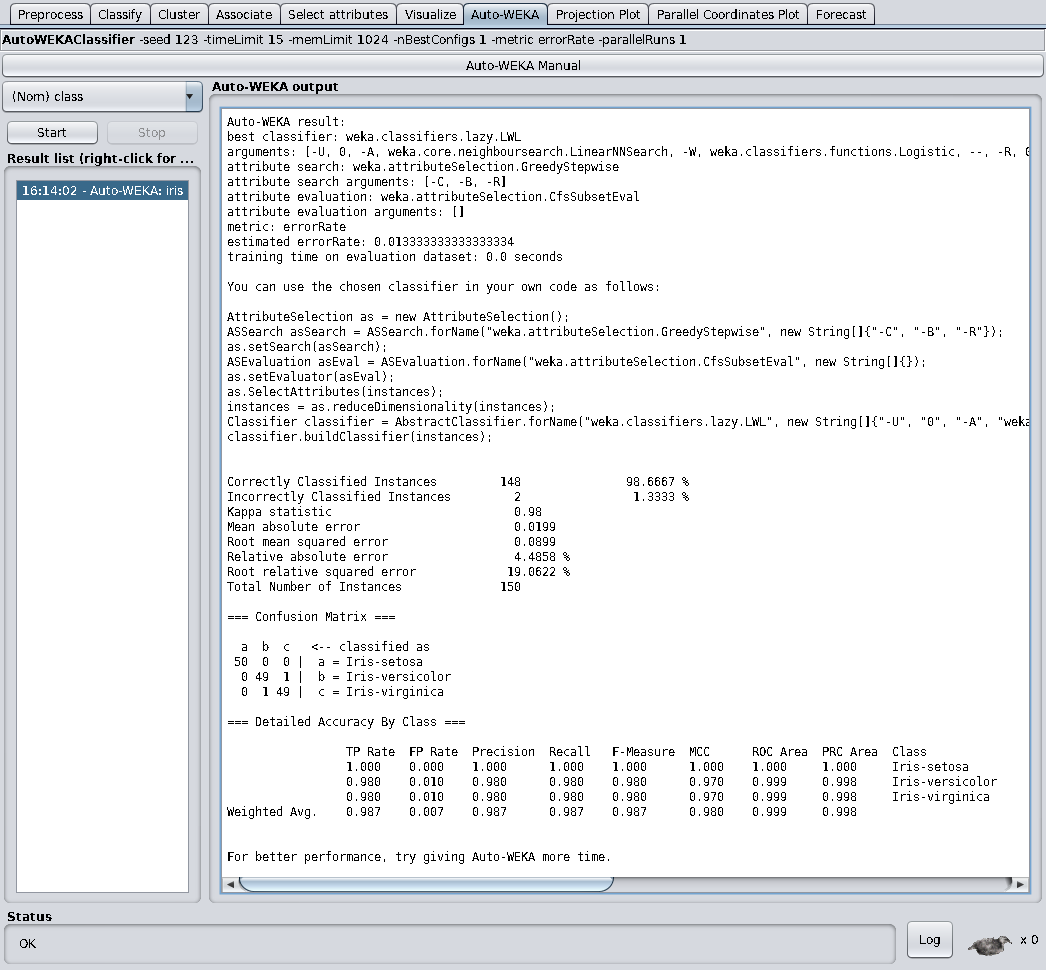
\includegraphics[width=\textwidth]{tab}
\caption{Auto-WEKA tab showing the output of a completed run.}
\label{fig:tab}
\end{center}
\end{figure}

Alternatively, Auto-WEKA can be run through the normal ``Classify'' panel by
selecting it from the list of classifiers (Figure~\ref{fig:classifier}).

\begin{figure}[!ht]
\begin{center}
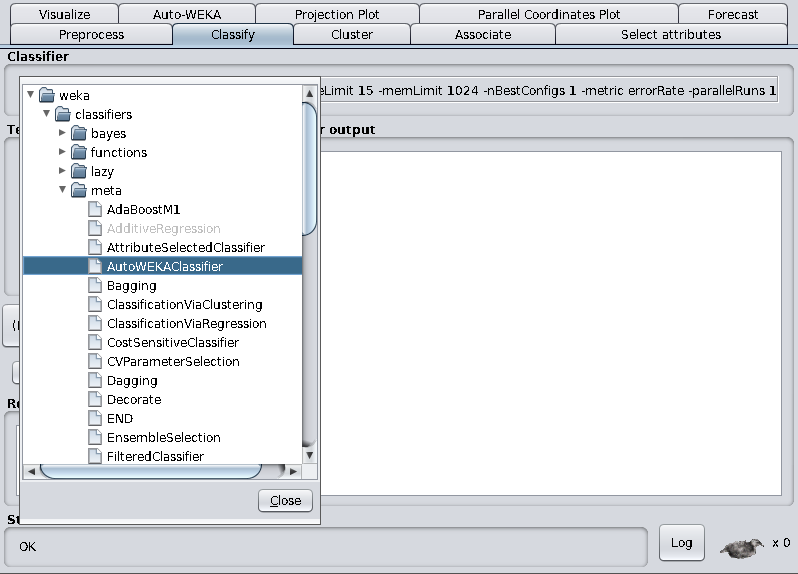
\includegraphics[width=\textwidth]{classifier}
\caption{Location of the Auto-WEKA classifier in the list of classifiers.}
\label{fig:classifier}
\end{center}
\end{figure}

When using Auto-WEKA like a normal classifier, it is important to select the
Test option ``Use training set''. Auto-WEKA performs a statistically rigorous
evaluation internally and does not require an external split into training and
test sets that WEKA provides. Not selecting this option will not improve the
quality of the result and cause Auto-WEKA to take much longer.
Figure~\ref{fig:train} shows the recommended setting.

\begin{figure}[!ht]
\begin{center}
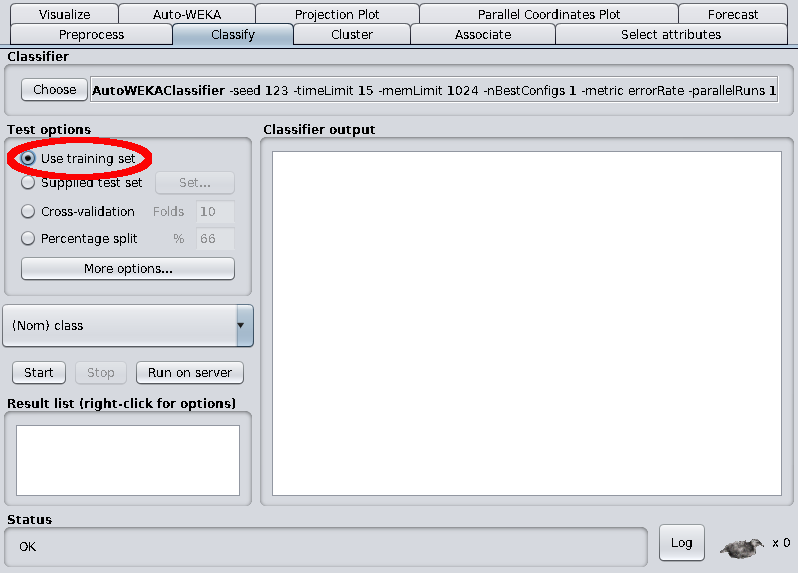
\includegraphics[width=\textwidth]{train}
\caption{Recommended evaluation setting when using Auto-WEKA like a normal
classifier.}
\label{fig:train}
\end{center}
\end{figure}

Auto-WEKA has only a few options. Figure~\ref{fig:options} shows them. Usually,
you can leave them at their default values. For most users, only two options are
relevant:
\begin{description}
\item[timeLimit] The time in minutes Auto-WEKA will take to determine the best
classifier and configuration. If you get bad results, try increasing this value.
\item[memLimit] The memory limit in Megabytes for running classifiers. If you
have a very large dataset, you may need to increase this value.
\end{description}

\begin{figure}[!ht]
\begin{center}
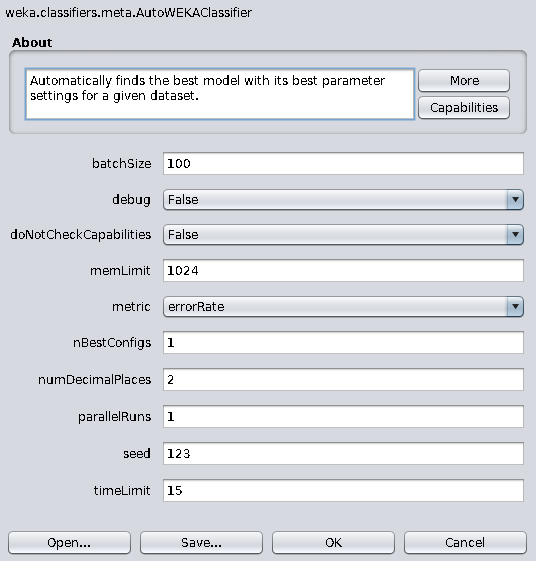
\includegraphics[width=\textwidth]{options}
\caption{Auto-WEKA options.}
\label{fig:options}
\end{center}
\end{figure}

While Auto-WEKA is running, it will provide the number of evaluated
configurations and estimated error of the best configuration found so far in the
status bar.

\medskip

Note that the time limit is \emph{approximate} and Auto-WEKA may not take
\emph{exactly} as long as requested.

%%%%%%%%%%%%%%%%%%%%%%%%%%%%%%%%%%%%%%%%%%% 
\subsection{Running Experiments Using the CLI}\label{sec:running}
%%%%%%%%%%%%%%%%%%%%%%%%%%%%%%%%%%%%%%%%%%%

Auto-WEKA can be run from the CLI like any other WEKA classifier, for example:
\begin{verbatim}
java -cp autoweka.jar weka.classifiers.meta.AutoWEKAClassifier \
    -t iris.arff -timeLimit 15 -no-cv
\end{verbatim}

Running Auto-WEKA with the \verb=-h= flag or without any options lists the
options that can be set by the user:
\begin{verbatim}
java -cp autoweka.jar weka.classifiers.meta.AutoWEKAClassifier -h

Help requested.

General options:

-h or -help
	Output help information.
-synopsis or -info
	Output synopsis for classifier (use in conjunction  with -h)
-t <name of training file>
	Sets training file.
-T <name of test file>
	Sets test file. If missing, a cross-validation will be performed
	on the training data.
-c <class index>
	Sets index of class attribute (default: last).
-x <number of folds>
	Sets number of folds for cross-validation (default: 10).
-no-cv
	Do not perform any cross validation.
-force-batch-training
	Always train classifier in batch mode, never incrementally.
-split-percentage <percentage>
	Sets the percentage for the train/test set split, e.g., 66.
-preserve-order
	Preserves the order in the percentage split.
-s <random number seed>
	Sets random number seed for cross-validation or percentage split
	(default: 1).
-m <name of file with cost matrix>
	Sets file with cost matrix.
-toggle <comma-separated list of evaluation metric names>
	Comma separated list of metric names to toggle in the output.
	All metrics are output by default with the exception of 'Coverage' and 'Region size'.
	Available metrics:
	Correct,Incorrect,Kappa,Total cost,Average cost,KB relative,KB information,
	Correlation,Complexity 0,Complexity scheme,Complexity improvement,
	MAE,RMSE,RAE,RRSE,Coverage,Region size,TP rate,FP rate,Precision,Recall,
	F-measure,MCC,ROC area,PRC area
-l <name of input file>
	Sets model input file. In case the filename ends with '.xml',
	a PMML file is loaded or, if that fails, options are loaded
	from the XML file.
-d <name of output file>
	Sets model output file. In case the filename ends with '.xml',
	only the options are saved to the XML file, not the model.
-v
	Outputs no statistics for training data.
-o
	Outputs statistics only, not the classifier.
-do-not-output-per-class-statistics
	Do not output statistics for each class.
-k
	Outputs information-theoretic statistics.
-classifications "weka.classifiers.evaluation.output.prediction.AbstractOutput + options"
	Uses the specified class for generating the classification output.
	E.g.: weka.classifiers.evaluation.output.prediction.PlainText
-p range
	Outputs predictions for test instances (or the train instances if
	no test instances provided and -no-cv is used), along with the 
	attributes in the specified range (and nothing else). 
	Use '-p 0' if no attributes are desired.
	Deprecated: use "-classifications ..." instead.
-distribution
	Outputs the distribution instead of only the prediction
	in conjunction with the '-p' option (only nominal classes).
	Deprecated: use "-classifications ..." instead.
-r
	Only outputs cumulative margin distribution.
-xml filename | xml-string
	Retrieves the options from the XML-data instead of the command line.
-threshold-file <file>
	The file to save the threshold data to.
	The format is determined by the extensions, e.g., '.arff' for ARFF 
	format or '.csv' for CSV.
-threshold-label <label>
	The class label to determine the threshold data for
	(default is the first label)
-no-predictions
	Turns off the collection of predictions in order to conserve memory.

Options specific to weka.classifiers.meta.AutoWEKAClassifier:

-seed <seed>
	The seed for the random number generator.
	(default: 123)
-timeLimit <limit>
	The time limit for tuning in minutes (approximately).
	(default: 15)
-memLimit <limit>
	The memory limit for runs in MiB.
	(default: 1024)
-nBestConfigs <limit>
	The amount of best configurations to return.
	(default: 1024)
-metric <metric>
	The metric to optimise.
	(default: errorRate)
-parallelRuns <runs>
	The number of parallel runs. EXPERIMENTAL, BE CAREFUL WHEN SETTING.
	(default: 1)
-output-debug-info
	If set, classifier is run in debug mode and
	may output additional info to the console
-do-not-check-capabilities
	If set, classifier capabilities are not checked before classifier is built
	(use with caution).
-num-decimal-places
	The number of decimal places for the output of numbers in the model (default 2).
-batch-size
	The desired batch size for batch prediction  (default 100).
\end{verbatim}

\subsection{Saving and Loading Models}

Once Auto-WEKA has been run, you can save the trained model to get predictions
on similar data. In the WEKA GUI, right-click on a run in the output list window
and select `Save model'. On the CLI, use the \verb=-d= flag. More information on
saving and loading models can be found on the WEKA wiki at
\url{https://weka.wikispaces.com/Saving+and+loading+models}.

The Auto-WEKA output also contains the Java code for creating an instance of the
classifier and attribute selection method that it found. This allows to retrain
the model on different data.

\section{Developer Documentation}

Auto-WEKA's internal structure is complex and comprises more than 10,000 lines
of code. A detailed explanation is beyond the scope of this document; more
details can be found in the Javadoc, available at
\url{https://automl.github.io/autoweka/}. A high-level overview of the internal
structure of Auto-WEKA is shown in Figure~\ref{fig:devel-overview}.

\begin{figure}[!ht]
\begin{center}
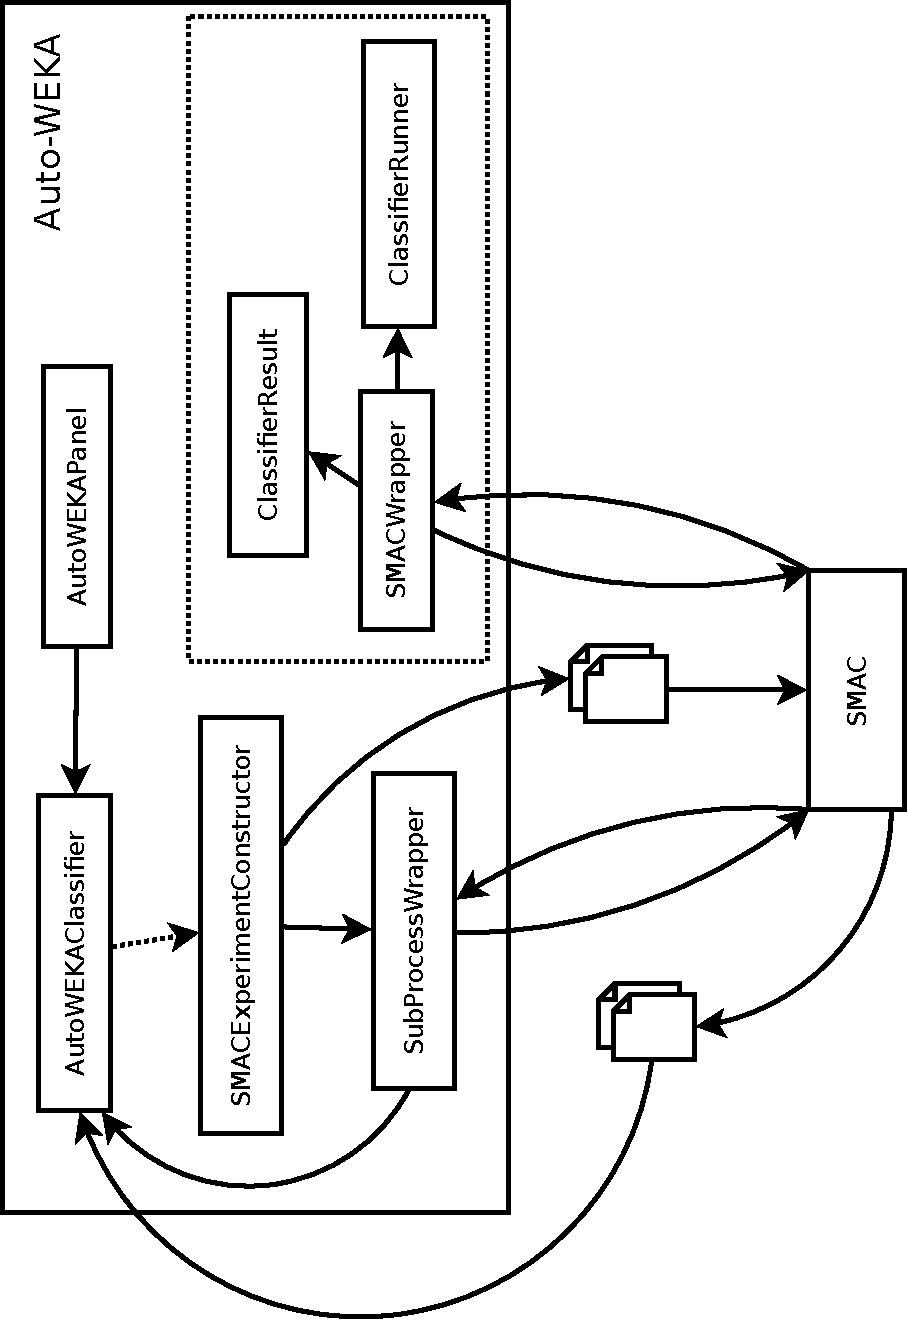
\includegraphics[angle=-90,width=\textwidth]{devel-overview-crop}
\caption{High-level overview of Auto-WEKA internal structure.}
\label{fig:devel-overview}
\end{center}
\end{figure}

The user interface of Auto-WEKA is defined in the \verb=AutoWEKAClassifier= and
\verb=AutoWEKAPanel= classes, where the latter defines the elements of the
custom Auto-WEKA panel and calls \verb=AutoWEKAClassifier=. New user options and
additional arguments should be specified there.

The SMAC optimization tool is called through the
\verb=SMACExperimentConstructor= and \verb=SubProcessWrapper= classes. The
former prepares a set of files that contain the data, the definition of the
parameter space, the training budget, and other information necessary for SMAC
to run. These files are created in the system's temporary directory in a folder
named \verb=autoweka<random number>=. The \verb=SubProcessWrapper= calls SMAC as
an external process and points it to these files.

SMAC then calls Auto-WEKA's \verb=SMACWrapper= class during the optimization
process to evaluate the performance of a classifier and its parameters. The
\verb=SMACWrapper= trains and evaluates the classifier with given parameters
with the \verb=ClassifierRunner= class, which creates a \verb=ClassifierResult=.
This information is passed back to SMAC.

After SMAC's optimization completes, control is passed back to Auto-WEKA, which
takes the information communicated directly from SMAC through its output and
parses result files that SMAC generated. This information is used to determine
the best classifier and its parameters, which is finally presented to the user.

\appendix

\section{Auto-WEKA Configuration Space}
\subsection{Classifiers, Parameters, and Parameter Ranges}
\begin{landscape}
\begin{longtabu} to \linewidth {XXXX}
\toprule
\rowfont\bfseries Classifier & Parameter & Value Range & Default\\
\\\midrule
\endhead
\multicolumn{4}{r}{continued\ldots}\\
\endfoot
\\\bottomrule
\endlastfoot
J48 & O & true, false & false\\
 & U & true, false & false\\
 & B & true, false & false\\
 & J & true, false & false\\
 & A & true, false & false\\
 & S & true, false & false\\
 & M & 1, 64 & 2\\
 & C & 0, 1 & 25\\
\midrule
DecisionTable & E & acc, rmse, mae, auc & acc\\
 & I & true, false & false\\
 & S & BestFirst, GreedyStepwise & BestFirst\\
 & X & 1, 2, 3, 4 & 1\\
\midrule
GaussianProcesses & L & 0001, 1 & 1\\
 & N & 0, 1, 2 & 0\\
 & K & NormalizedPolyKernel, PolyKernel, Puk, RBFKernel & NormalizedPolyKernel\\
 & E & 2, 5 & 0\\
 & L & true, false & false\\
 & E & 2, 5 & 0\\
 & L & true, false & false\\
 & S & 1, 10 & 0\\
 & O & 1, 1 & 0\\
 & C & 0001, 1 & 01\\
\midrule
M5P & N & true, false & false\\
 & M & 1, 64 & 4\\
 & U & true, false & false\\
 & R & true, false & false\\
\midrule
KStar & B & 1, 100 & 20\\
 & E & true, false & false\\
 & M & a, d, m, n & a\\
\midrule
LMT & B & true, false & false\\
 & R & true, false & false\\
 & C & true, false & false\\
 & P & true, false & false\\
 & M & 1, 64 & 15\\
 & W & 0 & 0\\
 & W & 0, 1 & 0\\
 & A & true, false & false\\
\midrule
PART & N & 2, 5 & 3\\
 & M & 1, 64 & 2\\
 & R & true, false & false\\
 & B & true, false & false\\
\midrule
SMO & C & 5, 5 & 0\\
 & N & 0, 1, 2 & 0\\
 & M & true, false & false\\
 & K & NormalizedPolyKernel, PolyKernel, Puk, RBFKernel & NormalizedPolyKernel\\
 & E & 2, 5 & 0\\
 & L & true, false & false\\
 & E & 2, 5 & 0\\
 & L & true, false & false\\
 & S & 1, 10 & 0\\
 & O & 1, 1 & 0\\
 & G & 0001, 1 & 01\\
\midrule
BayesNet & D & true, false & false\\
 & Q & K2, HillClimber, LAGDHillClimber, SimulatedAnnealing, TabuSearch, TAN & K2\\
\midrule
NaiveBayes & K & true, false & false\\
 & D & true, false & false\\
\midrule
JRip & N & 1, 5 & 0\\
 & E & true, false & false\\
 & P & true, false & false\\
 & O & 1, 5 & 2\\
\midrule
SimpleLogistic & S & true, false & false\\
 & W & 0 & 0\\
 & W & 0, 1 & 0\\
 & A & true, false & false\\
\midrule
LinearRegression & S & 0, 1, 2 & 0\\
 & C & true, false & false\\
 & R & 1e-7, 10 & 1e-7\\
\midrule
VotedPerceptron & I & 1, 10 & 1\\
 & M & 5000, 50000 & 10000\\
 & E & 2, 5 & 0\\
\midrule
SGD & F & 0, 1, 2 & 0\\
 & L & 00001, 1 & 01\\
 & R & 1e-12, 10 & 1e-4\\
 & N & true, false & false\\
 & M & true, false & false\\
\midrule
Logistic & R & 1e-12, 10 & 1e-7\\
\midrule
OneR & B & 1, 32 & 6\\
\midrule
MultilayerPerceptron & L & 1, 1 & 3\\
 & M & 1, 1 & 2\\
 & B & true, false & false\\
 & H & a, i, o, t & a\\
 & C & true, false & false\\
 & R & true, false & false\\
 & D & true, false & false\\
 & S & 1 & 1\\
\midrule
REPTree & M & 1, 64 & 2\\
 & V & 1e-5, 1e-1 & 1e-3\\
 & L & -1 & -1\\
 & L & 2, 20 & 2\\
 & P & true, false & false\\
\midrule
IBk & E & true, false & false\\
 & K & 1, 64 & 1\\
 & X & true, false & false\\
 & F & true, false & false\\
 & I & true, false & false\\
\midrule
M5Rules & N & true, false & false\\
 & M & 1, 64 & 4\\
 & U & true, false & false\\
 & R & true, false & false\\
\midrule
RandomForest & I & 2, 256 & 10\\
 & K & 0 & 0\\
 & K & 1, 32 & 2\\
 & depth & 0 & 0\\
 & depth & 1, 20 & 2\\
\midrule
RandomTree & M & 1, 64 & 1\\
 & K & 0 & 0\\
 & K & 2, 32 & 2\\
 & depth & 0 & 0\\
 & depth & 2, 20 & 2\\
 & N & 0 & 0\\
 & N & 2, 5 & 3\\
 & U & true, false & false\\
\midrule
SMOreg & C & 5, 5 & 0\\
 & N & 0, 1, 2 & 0\\
 & I & RegSMOImproved & RegSMOImproved\\
 & V & true, false & false\\
 & K & NormalizedPolyKernel, PolyKernel, Puk, RBFKernel & NormalizedPolyKernel\\
 & E & 2, 5 & 0\\
 & L & true, false & false\\
 & E & 2, 5 & 0\\
 & L & true, false & false\\
 & S & 1, 10 & 0\\
 & O & 1, 1 & 0\\
 & G & 0001, 1 & 01\\
\midrule
Vote & R & AVG, PROD, MAJ, MIN, MAX & AVG\\
 & S & 1 & 1\\
\midrule
Stacking & X & 10 & 10\\
 & S & 1 & 1\\
\midrule
Bagging & P & 10, 100 & 100\\
 & I & 2, 128 & 10\\
 & S & 1 & 1\\
 & O & true, false & false\\
\midrule
 & P & 100 & 100\\
 & P & 50, 100 & 100\\
 & I & 2, 128 & 10\\
 & Q & true, false & false\\
 & S & 1 & 1\\
\midrule
 & S & 1 & 1\\
 & S & 0, 0 & 1\\
 & I & 2, 128 & 10\\
\midrule
 & K & -1, 10, 30, 60, 90, 120 & -1\\
 & U & 0, 1, 2, 3, 4 & 0\\
 & A & LinearNNSearch & LinearNNSearch\\
\midrule
RandomSubSpace & I & 2, 64 & 10\\
 & P & 1, 0 & 5\\
 & S & 1 & 1\\
\midrule
AttributeSelectedClassifier & S & BestFirst, GreedyStepwise & BestFirst\\
 & E & CfsSubsetEval & CfsSubsetEval\\
\midrule
RandomCommittee & I & 2, 64 & 10\\
 & S & 1 & 1\\
\midrule
\end{longtabu}
\end{landscape}
\subsection{Attribute Searches, Parameters, and Parameter Ranges}
\begin{landscape}
\begin{longtabu} to \linewidth {XXXX}
\toprule
\rowfont\bfseries Attribute Search & Parameter & Value Range & Default\\
\\\midrule
\endhead
\multicolumn{4}{r}{continued\ldots}\\
\endfoot
\\\bottomrule
\endlastfoot
BestFirst & D & 0, 1, 2 & 1\\
 & N & 2, 10 & 5\\
\midrule
GreedyStepwise & C & true, false & false\\
 & B & true, false & false\\
 & R & true, false & false\\
 & N & 10, 1000 & 30\\
\midrule
\end{longtabu}
\end{landscape}
\subsection{Attribute Evaluations, Parameters, and Parameter Ranges}
\begin{landscape}
\begin{longtabu} to \linewidth {XXXX}
\toprule
\rowfont\bfseries Attribute Evaluation & Parameter & Value Range & Default\\
\\\midrule
\endhead
\multicolumn{4}{r}{continued\ldots}\\
\endfoot
\\\bottomrule
\endlastfoot
CfsSubsetEval & M & true, false & false\\
 & L & true, false & false\\
\midrule
\end{longtabu}
\end{landscape}


\end{document}
